\documentclass[UTF8]{ctexart}

\usepackage{amsmath, amssymb, amsthm}
\usepackage{mathrsfs}
\usepackage{graphicx}
\usepackage{float}
\usepackage{tikz}

% 图按章编号，并显示为“图 6-1”格式。
\numberwithin{figure}{section}
\renewcommand{\thefigure}{\thesection-\arabic{figure}}
\usepackage{tikz-cd}
\usepackage{pgfplots}
\usepackage{xltabular}
\usepackage{booktabs}
\usepackage{geometry}
\usepackage{extarrows}
\geometry{a4paper, margin=2cm}
\pgfplotsset{compat=1.18}
\usetikzlibrary{shapes.geometric, positioning, calc, decorations.pathreplacing, 3d}

\usepackage[numbers,square]{natbib}
\newcommand{\scite}[1]{\textsuperscript{\cite{#1}}}

\newtheorem{theorem}{定理}[subsection]
\newtheorem{proposition}[theorem]{命题}
\newtheorem{corollary}[theorem]{推论}
\newtheorem{lemma}[theorem]{引理}
\theoremstyle{definition}
\newtheorem{definition}[theorem]{定义}
\newtheoremstyle{examplestyle}{3pt}{3pt}{\itshape}{0pt}{\bfseries}{.}{.5em}{\thmnumber{例 \arabic{example}}\thmnote{\ (#3)}}
\theoremstyle{examplestyle}
\newtheorem{example}{}[subsection]
\theoremstyle{remark}
\newtheorem*{remark}{注}

\title{L1凸松弛压缩感知信号恢复}
\author{}
\date{}

\usepackage[hidelinks]{hyperref}

\begin{document}

\maketitle

\section{摘要}
\label{sec:abstract}

压缩感知理论指出，当信号具有稀疏性或可压缩性时，可以通过远低于奈奎斯特率的线性测量以高概率恢复原始信号。最直接的 L0 稀疏恢复问题是 NP-难的组合优化问题，本文引入 L1 凸松弛将其转化为凸优化问题，并围绕带噪声稀疏信号恢复展开研究。

本文不调用任何商用凸优化求解器，自主实现了 FISTA 加速近端梯度算法；针对约束形式 L1 恢复问题，设计了 $\lambda$ 几何递减序列与残差曲线插值策略，稳健匹配残差约束 $\delta$；同时采用解析伪逆作为 L2 最小范数基线，保证对比公平并降低计算开销。

在仿真实验中，本文系统分析了采样维度 $M$、稀疏度 $K$ 与噪声强度 $\sigma$ 对重建性能的影响。结果表明：观测维度存在明显的相变临界值，当 $M$ 超过临界值时支撑集恢复成功率快速趋近 $100\%$；噪声会抬升临界采样规模并降低重建精度；L1 凸松弛恢复效果显著优于 L2 最小范数基线。

\noindent\textbf{关键词：}压缩感知；L1 凸松弛；FISTA；稀疏恢复；相变现象；KKT 条件

\section{引言}
\label{sec:intro}

奈奎斯特采样定理指出，要无失真地重建带限信号，采样率不得低于信号最高频率的两倍。然而在许多实际场景中，信号本身具有稀疏性或可压缩性，传统均匀采样方式获取了大量冗余数据，采样与存储成本高昂。压缩感知理论表明，对于稀疏信号，可以通过远低于奈奎斯特率的线性测量以高概率精确恢复，其核心在于利用信号的稀疏结构~\scite{donoho2006}。

考虑 $K$-稀疏信号 $x\in\mathbb{R}^n$（即至多 $K$ 个非零分量），通过测量矩阵 $A\in\mathbb{R}^{M\times n}$（$M<n$）得到观测 $y=Ax$。理论上最直接的恢复模型是 L0 范数极小化
\[
\min_{x\in\mathbb{R}^n}\ \|x\|_0 \qquad \text{s.t.} \quad Ax=y,
\]
但该问题是 NP-难的组合优化问题，难以大规模精确求解。L1 凸松弛将 L0 范数替换为 L1 范数，得到凸优化问题，从而能够高效求解，并在一定条件下保证恢复精度~\scite{candes2006stable}。

在现有课程作业或朴素实现中，常见以下几类简化缺陷：
\begin{itemize}
\item 直接对正则参数 $\lambda$ 二分搜索，忽略残差函数 $r(\lambda)$ 单调非减但非严格单调、以及离散路径数值误差带来的失效风险；
\item L2 基线采用迭代梯度投影，收敛缓慢且引入额外数值误差；
\item 使用固定阈值 $|x_i|>\tau$ 判定支撑集，噪声环境下易漏判、误判；
\item 使用未加速的 ISTA，收敛速度慢，批量仿真耗时高。
\end{itemize}
本项目针对上述问题，设计并实现稳健的约束 L1 恢复方案：自研 FISTA 求解 LASSO，采用 $\lambda$ 几何序列与插值策略匹配残差约束，使用解析伪逆作为 L2 对照基线，并采用 Top-K 集合相等判定支撑集恢复成功率。

本项目的研究目标分为四层：
\begin{enumerate}
\item \textbf{理论}：推导约束优化模型的 KKT 条件，理解 L1 凸松弛的可行性与最优性；
\item \textbf{算法}：自研 FISTA 求解 LASSO，并设计稳健的 $\lambda$ 寻根策略实现约束形式 L1 恢复；
\item \textbf{实验}：定量分析观测维度 $M$、稀疏度 $K$、噪声强度 $\sigma$ 对重建性能的影响，观测相变现象；
\item \textbf{对比}：与解析 L2 最小范数基线进行对照，结合 RIP 理论分析仿真结果。
\end{enumerate}

\section{问题建模与凸优化理论基础}
本章研究带噪声稀疏信号恢复问题，依次建立信号观测模型、L0 稀疏恢复的 L1 凸松弛模型，推导其 KKT 条件，并给出对偶问题与强对偶性结论。

\subsection{信号观测模型}
\label{sec:observation}

研究问题为带噪声稀疏信号恢复。设原始信号 $x_{\mathrm{true}}\in\mathbb{R}^n$ 是 $K$-稀疏信号（即至多 $K$ 个非零分量），通过高斯随机测量矩阵 $A\in\mathbb{R}^{M\times n}$ 得到观测向量 $y\in\mathbb{R}^M$，观测过程受到高斯噪声 $e\sim\mathcal{N}(0,\sigma^2 I_M)$ 污染：
\begin{equation}
\label{eq:observation}
y = A x_{\mathrm{true}} + e, \qquad e\sim\mathcal{N}(0,\sigma^2 I_M).
\end{equation}
各符号含义见表~\ref{tab:notation}。

\begin{table}[htbp]
\centering
\begin{tabular}{ll}
\hline
符号 & 含义 \\
\hline
$x_{\mathrm{true}}\in\mathbb{R}^n$ & $K$-稀疏原始信号 \\
$A\in\mathbb{R}^{M\times n}$ & 高斯随机测量矩阵，$M<n$ \\
$e\in\mathbb{R}^M$ & 高斯观测噪声，$e\sim\mathcal{N}(0,\sigma^2I_M)$ \\
$y\in\mathbb{R}^M$ & 观测向量 \\
$K$ & 原始信号稀疏度 \\
$M$ & 观测维度 \\
\hline
\end{tabular}
\caption{符号说明}
\label{tab:notation}
\end{table}

\subsection{L0 稀疏恢复与 L1 凸松弛}
\label{sec:relaxation}

\paragraph*{无噪声 L0 恢复模型}
在无噪声情形下，稀疏恢复问题可写为如下 L0 范数极小化问题：
\begin{equation}
\label{eq:L0}
\min_{x\in\mathbb{R}^n}\ \|x\|_0 \qquad \text{s.t.} \quad Ax=y,
\end{equation}
其中 $\|x\|_0$ 表示向量 $x$ 中非零分量的个数。

\paragraph*{带噪声约束 L0 恢复模型}
现实观测必然含有噪声，等式约束 $Ax=y$ 无法严格满足，因此将其替换为残差约束 $\|Ax-y\|_2\le\delta$，得到带噪声约束的 L0 模型：
\begin{equation}
\label{eq:L0noisy}
\min_{x\in\mathbb{R}^n}\ \|x\|_0 \qquad \text{s.t.} \quad \|Ax-y\|_2\le\delta.
\end{equation}
然而，L0 范数非凸、不连续，对应的组合优化问题难以大规模精确求解，因此考虑将 L0 范数凸松弛为 L1 范数。

\paragraph*{L1 凸松弛问题}
将 \eqref{eq:L0noisy} 中的 $\|x\|_0$ 替换为 $\|x\|_1$，得到核心优化问题
\begin{equation}
\label{eq:P}
(P)\qquad \min_{x\in\mathbb{R}^n}\ \|x\|_1 \qquad \text{s.t.} \quad \|Ax-y\|_2\le\delta.
\end{equation}

\paragraph*{凸性论证}
问题 \eqref{eq:P} 中，目标函数 $\|x\|_1$ 是凸函数；约束函数 $\|Ax-y\|_2$ 是凸函数，因此可行域
\[
\{x\in\mathbb{R}^n : \|Ax-y\|_2\le\delta\}
\]
是凸集。于是问题 \eqref{eq:P} 是一个凸优化问题，其局部最优解等价于全局最优解~\scite{boyd2004}。

\paragraph*{噪声阈值 $\delta$ 的选取}
对于观测模型 \eqref{eq:observation}，残差向量
\[
r=Ax-y=A(x-x_{\mathrm{true}})-e.
\]
当 $x=x_{\mathrm{true}}$ 时，真实残差满足
\[
r_{\mathrm{true}}=-e\sim\mathcal{N}(0,\sigma^2 I_M).
\]
标准化得 $\frac{1}{\sigma}r_{\mathrm{true}}\sim\mathcal{N}(0,I_M)$，于是
\begin{equation}
\label{eq:chi2}
Z=\frac{1}{\sigma^2}\|r_{\mathrm{true}}\|_2^2=\frac{1}{\sigma^2}\|e\|_2^2\sim\chi^2(M).
\end{equation}
由卡方分布的高概率上界，可取
\begin{equation}
\label{eq:delta}
\delta=\sigma\sqrt{M+2\sqrt{2M}}.
\end{equation}
$\delta$ 的取值影响可行域大小：取得过小可能导致可行域为空，取得过大会使约束过于松弛，解过度稀疏、失真严重。

\subsection{KKT 条件推导}
\label{sec:kkt}

对于凸优化问题 \eqref{eq:P}，构造拉格朗日函数
\begin{equation}
\label{eq:Lagrangian}
L(x,\lambda)=\|x\|_1+\lambda\bigl(\|Ax-y\|_2-\delta\bigr), \qquad \lambda\ge0.
\end{equation}

由于 $\|x\|_1$ 在原点不可微，稳定性条件中的梯度应替换为次梯度。$\|x\|_1$ 的次微分为
\begin{equation}
\label{eq:subdiff}
\partial\|x\|_1=\bigl\{s\in\mathbb{R}^n : s_i\in\partial|x_i|,\ i=1,\dots,n\bigr\},
\end{equation}
其中
\begin{equation}
\label{eq:subdiff_component}
\partial|x_i|=
\begin{cases}
\{1\}, & x_i>0,\\
\{-1\}, & x_i<0,\\
[-1,1], & x_i=0.
\end{cases}
\end{equation}
当 $\|Ax-y\|_2\neq0$ 时，$\|Ax-y\|_2$ 可微，其次梯度即梯度
\begin{equation}
\label{eq:gradnorm}
\partial_x\|Ax-y\|_2=\frac{A^T(Ax-y)}{\|Ax-y\|_2}.
\end{equation}

因此，若 $x^*$ 是问题 \eqref{eq:P} 的最优解，则存在乘子 $\lambda^*\ge0$，使得如下 KKT 条件成立：
\begin{enumerate}
\item \textbf{稳定性条件（次梯度最优性）}：
\begin{equation}
\label{eq:kkt-stationarity}
-\lambda^*\frac{A^T(Ax^*-y)}{\|Ax^*-y\|_2}\in\partial\|x^*\|_1.
\end{equation}
\item \textbf{原问题可行}：
\[
\|Ax^*-y\|_2\le\delta.
\]
\item \textbf{对偶可行}：
\[
\lambda^*\ge0.
\]
\item \textbf{互补松弛}：
\begin{equation}
\label{eq:kkt-complementarity}
\lambda^*\bigl(\|Ax^*-y\|_2-\delta\bigr)=0.
\end{equation}
\end{enumerate}

互补松弛条件说明：若 $\lambda^*>0$，则必有 $\|Ax^*-y\|_2=\delta$，即最优解位于约束边界上，约束被激活；若 $\lambda^*=0$，则约束不起作用，问题退化为无约束极小化 $\|x\|_1$。在 Slater 条件成立时（见第~\ref{sec:dual} 节），上述 KKT 条件也是全局最优的充分条件。

\subsection{对偶问题与强对偶性}
\label{sec:dual}

\paragraph*{对偶函数推导}
由拉格朗日函数 \eqref{eq:Lagrangian}，定义对偶函数
\begin{equation}
\label{eq:dual-function}
g(\lambda)=\inf_{x\in\mathbb{R}^n}L(x,\lambda)
=-\lambda\delta+\inf_{x\in\mathbb{R}^n}\Bigl(\|x\|_1+\lambda\|Ax-y\|_2\Bigr), \qquad \lambda\ge0.
\end{equation}
利用范数的共轭表示 $\|z\|_2=\sup_{\|u\|_2\le1}u^Tz$，并交换 $\inf$ 与 $\sup$（由 Slater 条件保证其合理性），可得
\begin{equation}
\label{eq:dual-inf}
\inf_{x\in\mathbb{R}^n}\Bigl(\|x\|_1+\lambda\|Ax-y\|_2\Bigr)
=\sup_{\|u\|_2\le1}\Bigl(-\lambda u^Ty+\inf_{x\in\mathbb{R}^n}\bigl(\|x\|_1+\lambda(A^Tu)^Tx\bigr)\Bigr).
\end{equation}
由于
\[
\inf_{x\in\mathbb{R}^n}\bigl(\|x\|_1+z^Tx\bigr)=
\begin{cases}
0, & \|z\|_\infty\le1,\\
-\infty, & \text{否则},
\end{cases}
\]
令 $v=\lambda u$，则
\begin{equation}
\label{eq:dual-g}
g(\lambda)=-\lambda\delta+\sup_{\|v\|_2\le\lambda,\ \|A^Tv\|_\infty\le1}\bigl(-v^Ty\bigr).
\end{equation}
于是拉格朗日对偶问题为
\begin{equation}
\label{eq:dual-max}
\max_{\lambda\ge0}\ g(\lambda)
=\max_{\lambda\ge0,\ \|v\|_2\le\lambda,\ \|A^Tv\|_\infty\le1}\Bigl(-\delta\lambda-v^Ty\Bigr).
\end{equation}
对固定的 $v$，由于 $\delta>0$，最优的 $\lambda$ 取 $\lambda=\|v\|_2$，故 \eqref{eq:dual-max} 等价于
\begin{equation}
\label{eq:dual-min}
\min_{v\in\mathbb{R}^M}\ y^Tv+\delta\|v\|_2 \qquad \text{s.t.} \quad \|A^Tv\|_\infty\le1.
\end{equation}
记 \eqref{eq:dual-min} 的最优值为 $q^*$，拉格朗日对偶问题 \eqref{eq:dual-max} 的最优值为 $d^*$，则有 $d^*=-q^*$；强对偶成立时，原问题最优值 $p^*$ 满足 $p^*=d^*=-q^*$。

\paragraph*{Slater 条件验证}
约束函数 $\|Ax-y\|_2$ 是凸函数。当 $\delta>0$ 且 $A$ 行满秩时（高斯随机矩阵以概率 $1$ 行满秩），方程 $Ax=y$ 有解，因此存在严格可行点 $x$ 满足 $\|Ax-y\|_2=0<\delta$，Slater 条件成立。当 $\delta=0$（即无噪声情形）时，可行域退化为仿射集 $\{x:Ax=y\}$，强对偶性仍可由线性约束凸优化理论保证，也可视为 $\delta\downarrow0$ 的极限情形。

\paragraph*{强对偶结论}
综上，问题 \eqref{eq:P} 满足约束规格，强对偶成立，原问题与对偶问题之间存在确定的最优值对应关系；这一性质为后续设计自研求解器与验证最优性提供了理论基础。

\section{自研求解器：加速近端梯度算法（FISTA）}
本章针对约束问题 \eqref{eq:P}，给出其等价 LASSO 形式与 $\lambda$ 寻根策略，推导近端算子与软阈值公式，并建立 ISTA/FISTA 迭代算法及收敛性分析。

\subsection{约束问题等价转化与 $\lambda$ 寻根策略}
\label{sec:lambda-root}

原约束问题 \eqref{eq:P} 可等价地表述为：存在参数 $\lambda>0$，使得 LASSO 问题
\begin{equation}
\label{eq:lasso}
\min_{x\in\mathbb{R}^n}\ \frac{1}{2}\|Ax-y\|_2^2+\lambda\|x\|_1
\end{equation}
的最优解 $x_\lambda$ 同时满足残差约束
\[
\|Ax_\lambda-y\|_2=\delta.
\]
残差函数 $r(\lambda)=\|Ax_\lambda-y\|_2$ 关于 $\lambda$ 单调非减，但可能存在非严格单调区间；在有限迭代和离散 $\lambda$-path 下，直接求解精确 $\lambda$ 还存在数值误差，因此采用几何路径 + 插值策略：构造 $\lambda$ 的几何递减序列，上限取 $\|A^Ty\|_\infty$，下限取 $10^{-6}\|A^Ty\|_\infty$；对每个 $\lambda$ 求解 LASSO \eqref{eq:lasso}，得到残差曲线 $r(\lambda)$，再利用插值方法寻找满足 $r(\lambda)=\delta$ 的目标 $\lambda$。

\subsection{近端算子理论推导}
\label{sec:prox}

对于闭凸函数 $f:\mathbb{R}^n\to(-\infty,+\infty]$，给定参数 $\tau>0$，近端算子定义为
\begin{equation}
\label{eq:prox-def}
\operatorname{prox}_{\tau f}(v)=\operatorname*{arg\,min}_{x\in\mathbb{R}^n}\left\{f(x)+\frac{1}{2\tau}\|x-v\|_2^2\right\}.
\end{equation}
其含义是在尽量保持 $x$ 接近 $v$ 的同时使 $f(x)$ 尽量小。

对 LASSO 问题 \eqref{eq:lasso}，令
\[
g(x)=\frac{1}{2}\|Ax-y\|_2^2,\qquad h(x)=\lambda\|x\|_1,
\]
则目标函数为 $g(x)+h(x)$，其中 $g$ 可微、$h$ 不可微但凸。采用“梯度下降处理 $g$、近端算子处理 $h$”的策略。

考虑 $h(x)=\lambda\|x\|_1$，由定义 \eqref{eq:prox-def} 得
\begin{equation}
\label{eq:prox-l1}
\operatorname{prox}_{\tau h}(v)=\operatorname*{arg\,min}_{x\in\mathbb{R}^n}\left\{\tau\lambda\|x\|_1+\frac{1}{2}\|x-v\|_2^2\right\}.
\end{equation}
将目标函数写开：
\[
\frac{1}{2}\|x-v\|_2^2+\tau\lambda\|x\|_1
=\sum_{i=1}^n\left[\frac{1}{2}(x_i-v_i)^2+\tau\lambda|x_i|\right].
\]
因此 $n$ 维问题可分解为 $n$ 个独立的一维问题。对标量问题
\[
\min_{u\in\mathbb{R}}\ \phi(u)=\frac{1}{2}(u-v)^2+\alpha|u|,
\]
其中记 $\alpha=\tau\lambda$。由于 $|u|$ 在 $0$ 处不可微，分情况讨论：
\begin{itemize}
\item 若 $u>0$，则 $\phi(u)=\frac{1}{2}(u-v)^2+\alpha u$，令 $\phi'(u)=u-v+\alpha=0$，得 $u^*=v-\alpha$，需满足 $v>\alpha$；
\item 若 $u<0$，则 $\phi(u)=\frac{1}{2}(u-v)^2-\alpha u$，令 $\phi'(u)=u-v-\alpha=0$，得 $u^*=v+\alpha$，需满足 $v<-\alpha$；
\item 若 $u=0$，由次梯度 $\partial|u|\big|_{u=0}=[-1,1]$，最优性条件 $0\in\partial\phi(0)=-v+\alpha[-1,1]$，即 $-\alpha\le v\le\alpha$。
\end{itemize}
综合得分段解
\begin{equation}
\label{eq:soft-threshold-scalar}
u^*=
\begin{cases}
v-\alpha, & v>\alpha,\\
0, & |v|\le\alpha,\\
v+\alpha, & v<-\alpha.
\end{cases}
\end{equation}
回代 $\alpha=\tau\lambda$ 并写成符号函数形式，即得软阈值算子
\begin{equation}
\label{eq:soft-threshold}
S_{\tau\lambda}(v)=\operatorname{sign}(v)\max\{|v|-\tau\lambda,0\}.
\end{equation}
对向量逐元素作用，有
\begin{equation}
\label{eq:prox-l1-closed}
\operatorname{prox}_{\tau\lambda\|\cdot\|_1}(v)=\bigl(S_{\tau\lambda}(v_1),\dots,S_{\tau\lambda}(v_n)\bigr)^T.
\end{equation}

\subsection{ISTA 与 FISTA 迭代算法}
\label{sec:ista-fista}

\paragraph*{近端梯度迭代格式}
对光滑部分 $g$ 在 $x_k$ 处作一阶近似，并加上邻近项以保证数值稳定性：
\begin{equation}
\label{eq:ista-update}
x_{k+1}=\operatorname*{arg\,min}_{x\in\mathbb{R}^n}\left\{g(x_k)+\nabla g(x_k)^T(x-x_k)+\frac{1}{2t}\|x-x_k\|_2^2+h(x)\right\},
\end{equation}
其中 $t>0$ 为步长。配方并略去与 $x$ 无关的常数项，可得
\[
x_{k+1}=\operatorname{prox}_{th}\bigl(x_k-t\nabla g(x_k)\bigr).
\]
对于 $h(x)=\lambda\|x\|_1$，有 $\operatorname{prox}_{th}(v)=S_{t\lambda}(v)$，且 $\nabla g(x)=A^T(Ax-y)$，因此 ISTA 迭代格式为
\begin{equation}
\label{eq:ista}
x_{k+1}=S_{t\lambda}\bigl(x_k-tA^T(Ax_k-y)\bigr).
\end{equation}
步长取 $0<t\le1/L$，其中 $L=\|A\|_2^2$ 是 $\nabla g$ 的 Lipschitz 常数，见下文收敛性分析。

\paragraph*{FISTA 加速}
ISTA 每一步只利用当前点 $x_k$ 的信息，收敛速度较慢。FISTA 引入 Nesterov 外推点 $y_k$ 加速：
\begin{equation}
\label{eq:fista-y}
x_{k+1}=\operatorname{prox}_{th}\bigl(y_k-t\nabla g(y_k)\bigr).
\end{equation}
辅助序列 $t_k$ 与外推点更新为
\begin{equation}
\label{eq:fista-t}
t_{k+1}=\frac{1+\sqrt{1+4t_k^2}}{2},
\end{equation}
\begin{equation}
\label{eq:fista-extrap}
y_{k+1}=x_{k+1}+\frac{t_k-1}{t_{k+1}}(x_{k+1}-x_k).
\end{equation}
通常取初值 $t_1=1$、$y_1=x_0$。FISTA 在目标函数值意义下具有 $O(1/k^2)$ 的收敛率~\scite{beck2009}，相比 ISTA 的 $O(1/k)$（见后文ISTA收敛性） 有本质加速。

\paragraph*{步长选取}
$g$ 的梯度 Lipschitz 常数为
\[
\|\nabla g(x)-\nabla g(z)\|_2=\|A^TA(x-z)\|_2\le\|A^TA\|_2\|x-z\|_2,
\]
故 $L=\|A^TA\|_2=\|A\|_2^2$。步长可取 $t=1/L=1/\|A\|_2^2$，其中 $\|A\|_2^2$ 通过计算 $A^TA$ 的最大特征值得到。

\paragraph*{ISTA 收敛性}
设 $x^*$ 为问题 \eqref{eq:lasso} 的最优解，$F(x)=g(x)+h(x)$。由 $g$ 的 Lipschitz 梯度性质，当 $t\le1/L$ 时，
\begin{equation}
\label{eq:descent-lemma}
g(x)\le g(z)+\nabla g(z)^T(x-z)+\frac{1}{2t}\|x-z\|_2^2.
\end{equation}
定义代理函数
\begin{equation}
\label{eq:Q}
Q_t(x,z)=g(z)+\nabla g(z)^T(x-z)+\frac{1}{2t}\|x-z\|_2^2+h(x),
\end{equation}
则 $F(x)\le Q_t(x,z)$，且 ISTA 更新 \eqref{eq:ista} 等价于 $x_{k+1}=\arg\min_x Q_t(x,x_k)$。由最优性条件，存在 $s_{k+1}\in\partial h(x_{k+1})$ 使得
\[
\nabla g(x_k)+\frac{1}{t}(x_{k+1}-x_k)+s_{k+1}=0.
\]
由 $h$ 的凸性可得
\[
h(x_{k+1})-h(x)\le-\nabla g(x_k)^T(x_{k+1}-x)-\frac{1}{t}(x_{k+1}-x_k)^T(x_{k+1}-x),
\]
由 $g$ 的凸性与 \eqref{eq:descent-lemma} 可得
\[
g(x_{k+1})-g(x)\le\nabla g(x_k)^T(x_{k+1}-x)+\frac{1}{2t}\|x_{k+1}-x_k\|_2^2.
\]
两式相加并利用恒等式
\[
2(a-b)^T(a-c)=\|a-b\|_2^2+\|a-c\|_2^2-\|b-c\|_2^2
\]
整理得
\begin{equation}
\label{eq:ista-key}
F(x_{k+1})-F(x)\le\frac{1}{2t}\left(\|x_k-x\|_2^2-\|x_{k+1}-x\|_2^2\right).
\end{equation}
令 $x=x^*$ 并对 $k=0,\dots,N-1$ 求和，利用 Telescoping 求和得
\[
\sum_{k=0}^{N-1}\bigl(F(x_{k+1})-F^*\bigr)\le\frac{1}{2t}\|x_0-x^*\|_2^2.
\]
又因 $F(x_k)$ 单调不增，故
\[
F(x_N)-F^*\le\frac{1}{N}\sum_{k=0}^{N-1}\bigl(F(x_{k+1})-F^*\bigr)\le\frac{\|x_0-x^*\|_2^2}{2tN}.
\]
因此
\begin{equation}
\label{eq:ista-rate}
F(x_N)-F^*=O\left(\frac{1}{N}\right),
\end{equation}
即 ISTA 具有 $O(1/k)$ 收敛率。

\paragraph*{停机准则}
采用双重停机准则：
\begin{itemize}
\item 相对迭代变化：
\[
r_x^{(k)}=\frac{\|x_{k+1}-x_k\|_2}{\max(1,\|x_k\|_2)}<10^{-5};
\]
\item 相对目标函数变化：
\[
r_F^{(k)}=\frac{|F_{k+1}-F_k|}{\max(1,|F_k|)}<10^{-8};
\]
\item 当迭代次数达到 $k_{\max}=500$ 时强制停机。
\end{itemize}
前两项同时满足时认为算法收敛；若达到最大迭代次数仍未满足，则强制终止并保留当前迭代解。

\subsection{L2 基线求解方案}
\label{sec:l2-baseline}

为了公平对比 L1 凸松弛方法的效果，本节实现一个 L2 最小范数基线求解器。其对比优化模型为
\begin{equation}
\label{eq:L2-baseline}
\min_{x\in\mathbb{R}^n}\ \|x\|_2 \qquad \text{s.t.} \quad \|Ax-y\|_2\le\delta.
\end{equation}
该模型不利用稀疏性，仅寻找能量最小的可行解，作为实验中的朴素对照。

\paragraph*{解析伪逆闭式解}
需要说明的是，问题 \eqref{eq:L2-baseline} 的最优解通常位于可行域边界 $\|Ax-y\|_2=\delta$ 上，并不等于等式约束 $Ax=y$ 下的最小范数解。但在欠定情形 $M<n$ 且 $A$ 行满秩时，$Ax=y$ 有解，此时可取等式约束最小范数解
\begin{equation}
\label{eq:l2-pinv}
\hat{x}_{L2}=A^T(AA^T)^{-1}y
\end{equation}
作为 L2 基线的简化实现。该解残差为零，恒满足 $\|A\hat{x}_{L2}-y\|_2\le\delta$，因而是 \eqref{eq:L2-baseline} 的一个可行解；虽然它不一定是最优解，但不利用稀疏性、计算简单、对比公平，足以作为朴素对照。相比原始方案中的梯度投影迭代，解析伪逆具有以下优点：
\begin{itemize}
\item 闭式求解，计算开销低；
\item 不引入迭代收敛误差，保证对比公平；
\item 在欠定行满秩情形下，伪逆解恒满足残差约束 $\|A\hat{x}_{L2}-y\|_2\le\delta$。
\end{itemize}

\paragraph*{可行性讨论}
当 $A$ 行满秩时，$Ax=y$ 有解，因此 $\hat{x}_{L2}$ 的残差为零，对任意 $\delta\ge0$ 均可行。若因数值或退化情形导致残差超过 $\delta$，理论上可启用投影策略，但本实验场景直接使用解析解，以保证 L2 基线的实现简单且公平。

\section{仿真实验方案设计}
本章规定批量仿真实验的完整方案，包括参数网格、噪声阈值、评价指标、单次实验流程与数据保存方式，为后续实验运行和结果分析提供统一标准。

\subsection{实验参数汇总}
\label{sec:params}

固定参数：信号长度 $n=128$。变量网格如表~\ref{tab:params} 所示。

\begin{table}[htbp]
\centering
\begin{tabular}{ll}
\hline
参数 & 取值 \\
\hline
观测维度 $M$ & $20,30,40,50,60,70,80,90,100$ \\
稀疏度 $K$ & $3,5,8,12,16,20$ \\
噪声标准差 $\sigma$ & $0,0.02,0.05,0.10$ \\
每组随机试验次数 & $50$ \\
\hline
\end{tabular}
\caption{实验参数网格}
\label{tab:params}
\end{table}

每组参数 $(M,K,\sigma)$ 独立重复 $50$ 次随机试验。

\subsection{噪声阈值 $\delta$ 选取规则}
\label{sec:delta-rule}

由第~\ref{sec:observation} 节的分析，取
\begin{equation}
\label{eq:delta-experiment}
\delta=\sigma\sqrt{M+2\sqrt{2M}}.
\end{equation}
该阈值来自卡方分布 $\chi^2(M)$ 的高概率上界，使真实残差以较高概率满足约束。$\delta$ 的取值影响可行域大小：取得过小可能导致可行域为空；取得过大会使约束过于松弛，解过度稀疏、失真严重。特别地，当 $\sigma=0$ 时 $\delta=0$，对应无噪声情形下的精确约束 $Ax=y$。

\subsection{评价指标定义}
\label{sec:metrics}

\paragraph*{支撑集恢复成功率}
已知真实稀疏度 $K$。对重建向量 $\hat{x}$，取绝对值最大的前 $K$ 个坐标构成估计支撑集
\begin{equation}
\label{eq:estimated-support}
\hat{S}=\operatorname*{arg\,max}_{|S|=K}\sum_{i\in S}|\hat{x}_i|,
\end{equation}
即若
\[
|\hat{x}_{i_1}|\ge|\hat{x}_{i_2}|\ge\cdots\ge|\hat{x}_{i_K}|\ge\max_{j\notin\hat{S}}|\hat{x}_j|,
\]
则
\[
\hat{S}=\{i_1,i_2,\dots,i_K\}.
\]
将估计支撑集 $\hat{S}$ 与真实支撑集 $S_{\mathrm{true}}$ 做集合相等判定，单次试验成功当且仅当 $\hat{S}=S_{\mathrm{true}}$。\emph{禁止使用固定阈值} $|\hat{x}_i|>\tau$ 判定支撑集，因为噪声环境下固定阈值会产生漏判和误判。

\paragraph*{相对重建误差}
相对重建误差定义为
\begin{equation}
\label{eq:re}
RE=\frac{\|\hat{x}-x_{\mathrm{true}}\|_2}{\|x_{\mathrm{true}}\|_2}.
\end{equation}
$RE$ 仅作为连续量化指标，不作为支撑集成功判定标准。

\subsection{单次完整实验流程}
\label{sec:single-run}

对每一组参数 $(M,K,\sigma)$ 和每一次随机试验，按以下步骤执行：
\begin{enumerate}
\item 生成 $K$-稀疏原始信号 $x_{\mathrm{true}}\in\mathbb{R}^n$：随机选取 $K$ 个支撑位置，非零分量独立服从标准正态分布；
\item 生成高斯随机测量矩阵 $A\in\mathbb{R}^{M\times n}$，元素独立服从标准正态分布；
\item 生成高斯噪声 $e\sim\mathcal{N}(0,\sigma^2I_M)$，构造观测向量
\[
y=Ax_{\mathrm{true}}+e;
\]
\item 按 \eqref{eq:delta-experiment} 计算 $\delta$，使用第~\ref{sec:lambda-root} 节的 FISTA+LASSO 路径插值方法求解约束 L1 恢复问题 \eqref{eq:P}，得到 $\hat{x}_{L1}$；
\item 使用第~\ref{sec:l2-baseline} 节的解析伪逆最小范数解作为 L2 基线（等式约束近似）
\[
\hat{x}_{L2}=A^T(AA^T)^{-1}y;
\]
\item 分别计算 $\hat{x}_{L1}$、$\hat{x}_{L2}$ 的支撑集恢复结果与相对重建误差 \eqref{eq:re}；
\item 重复上述过程 $50$ 次，统计支撑集恢复成功率与平均相对重建误差。
\end{enumerate}

\subsection{统计量与数据保存}
\label{sec:stats-save}

对每组参数 $(M,K,\sigma)$，统计以下指标：
\begin{itemize}
\item 支撑集恢复成功率：$50$ 次试验中 $\hat{S}=S_{\mathrm{true}}$ 的次数占比；
\item 平均相对重建误差：$50$ 次试验的 $RE$ 均值，L1 与 L2 分别统计。
\end{itemize}
将最终统计结果保存为 \texttt{.npy} 文件，避免重复运算。

\subsection{代码实现模块}
\label{sec:code-modules}

实验代码按以下模块组织：
\begin{itemize}
\item \texttt{FISTA.py}：自研 FISTA 求解 LASSO；
\item \texttt{lasso.py}：基于 FISTA 的 $\lambda$ 几何序列与插值寻根，求解约束 L1 问题；
\item \texttt{l2\_baseline.py}：L2 基线解析伪逆求解；
\item \texttt{experiment.py}：参数网格三层循环、$50$ 次随机试验、指标统计与结果保存。
\end{itemize}



\section{实验结果可视化}
\label{sec:visualization}

本章展示四类实验结果图表：无噪声相变热力图、支撑恢复成功率随观测维度变化折线图、L1 与 L2 平均相对重建误差对比图，以及单次样例恢复对照图。

\begin{figure}[H]
\centering
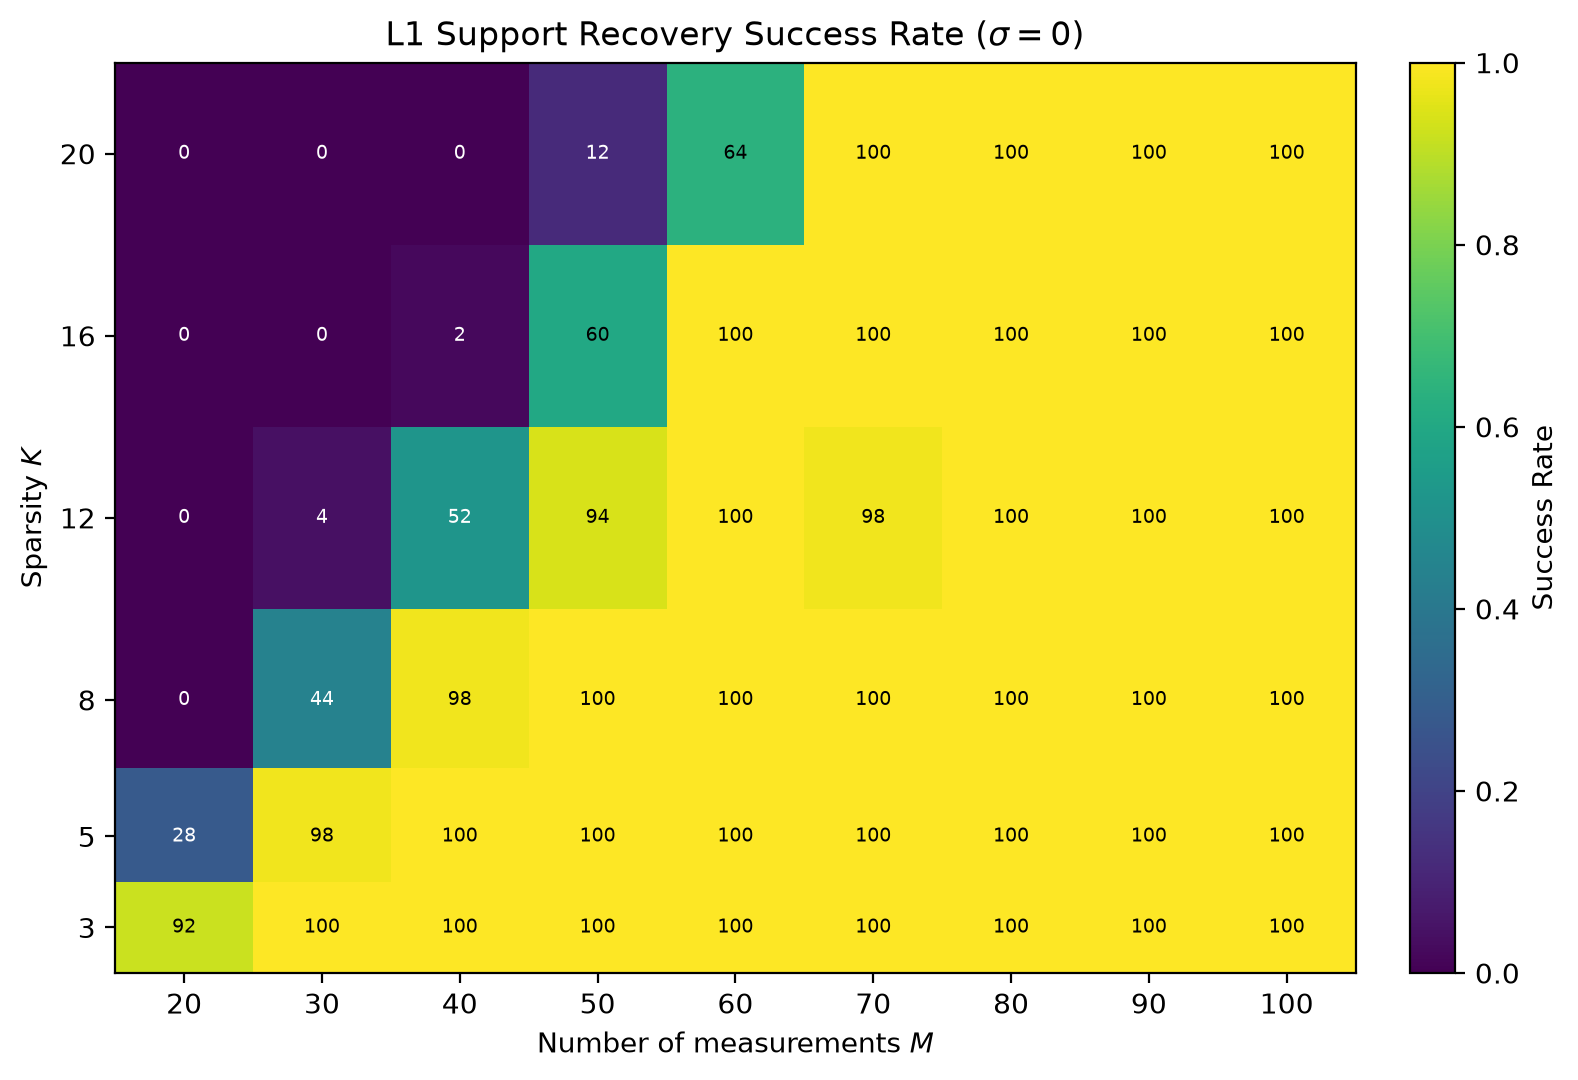
\includegraphics[width=0.72\textwidth]{figures/fig1_heatmap_sigma0.png}
\caption{无噪声情形（$\sigma=0$）下 L1 支撑集恢复成功率热力图}
\label{fig:heatmap}
\end{figure}

\begin{figure}[H]
\centering
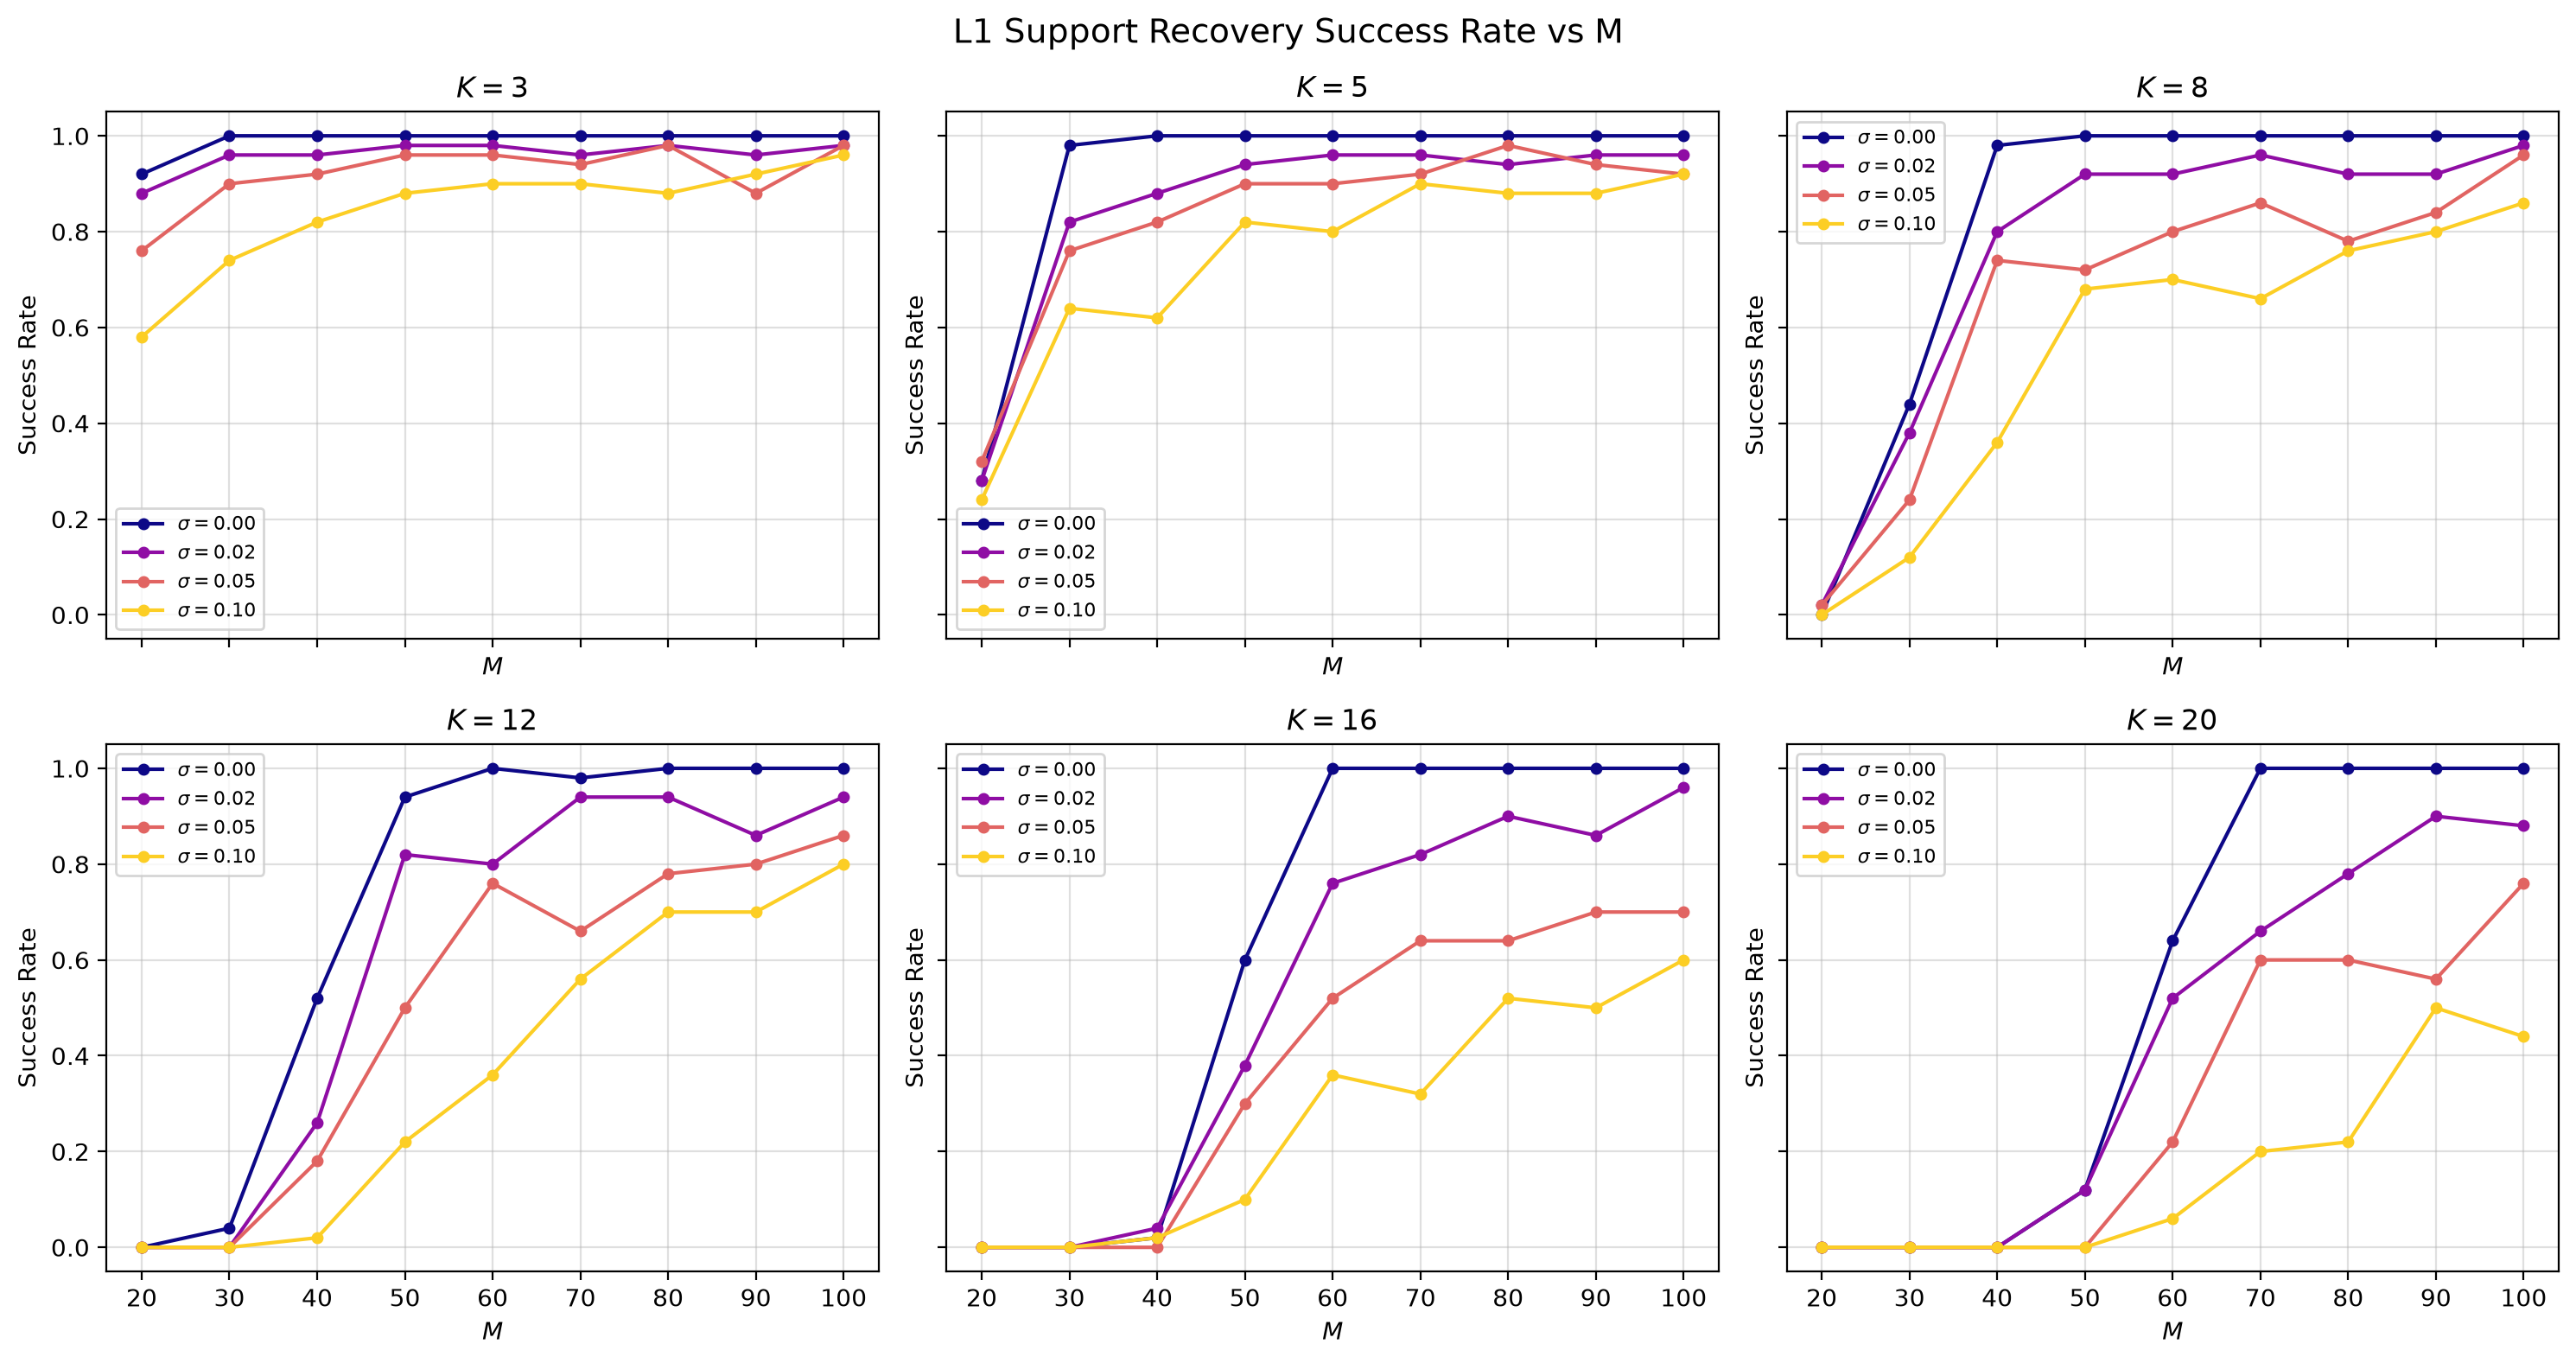
\includegraphics[width=0.98\textwidth]{figures/fig2_success_vs_M.png}
\caption{不同稀疏度 $K$ 与噪声强度 $\sigma$ 下，L1 支撑集恢复成功率随观测维度 $M$ 的变化}
\label{fig:success-vs-M}
\end{figure}

\begin{figure}[H]
\centering
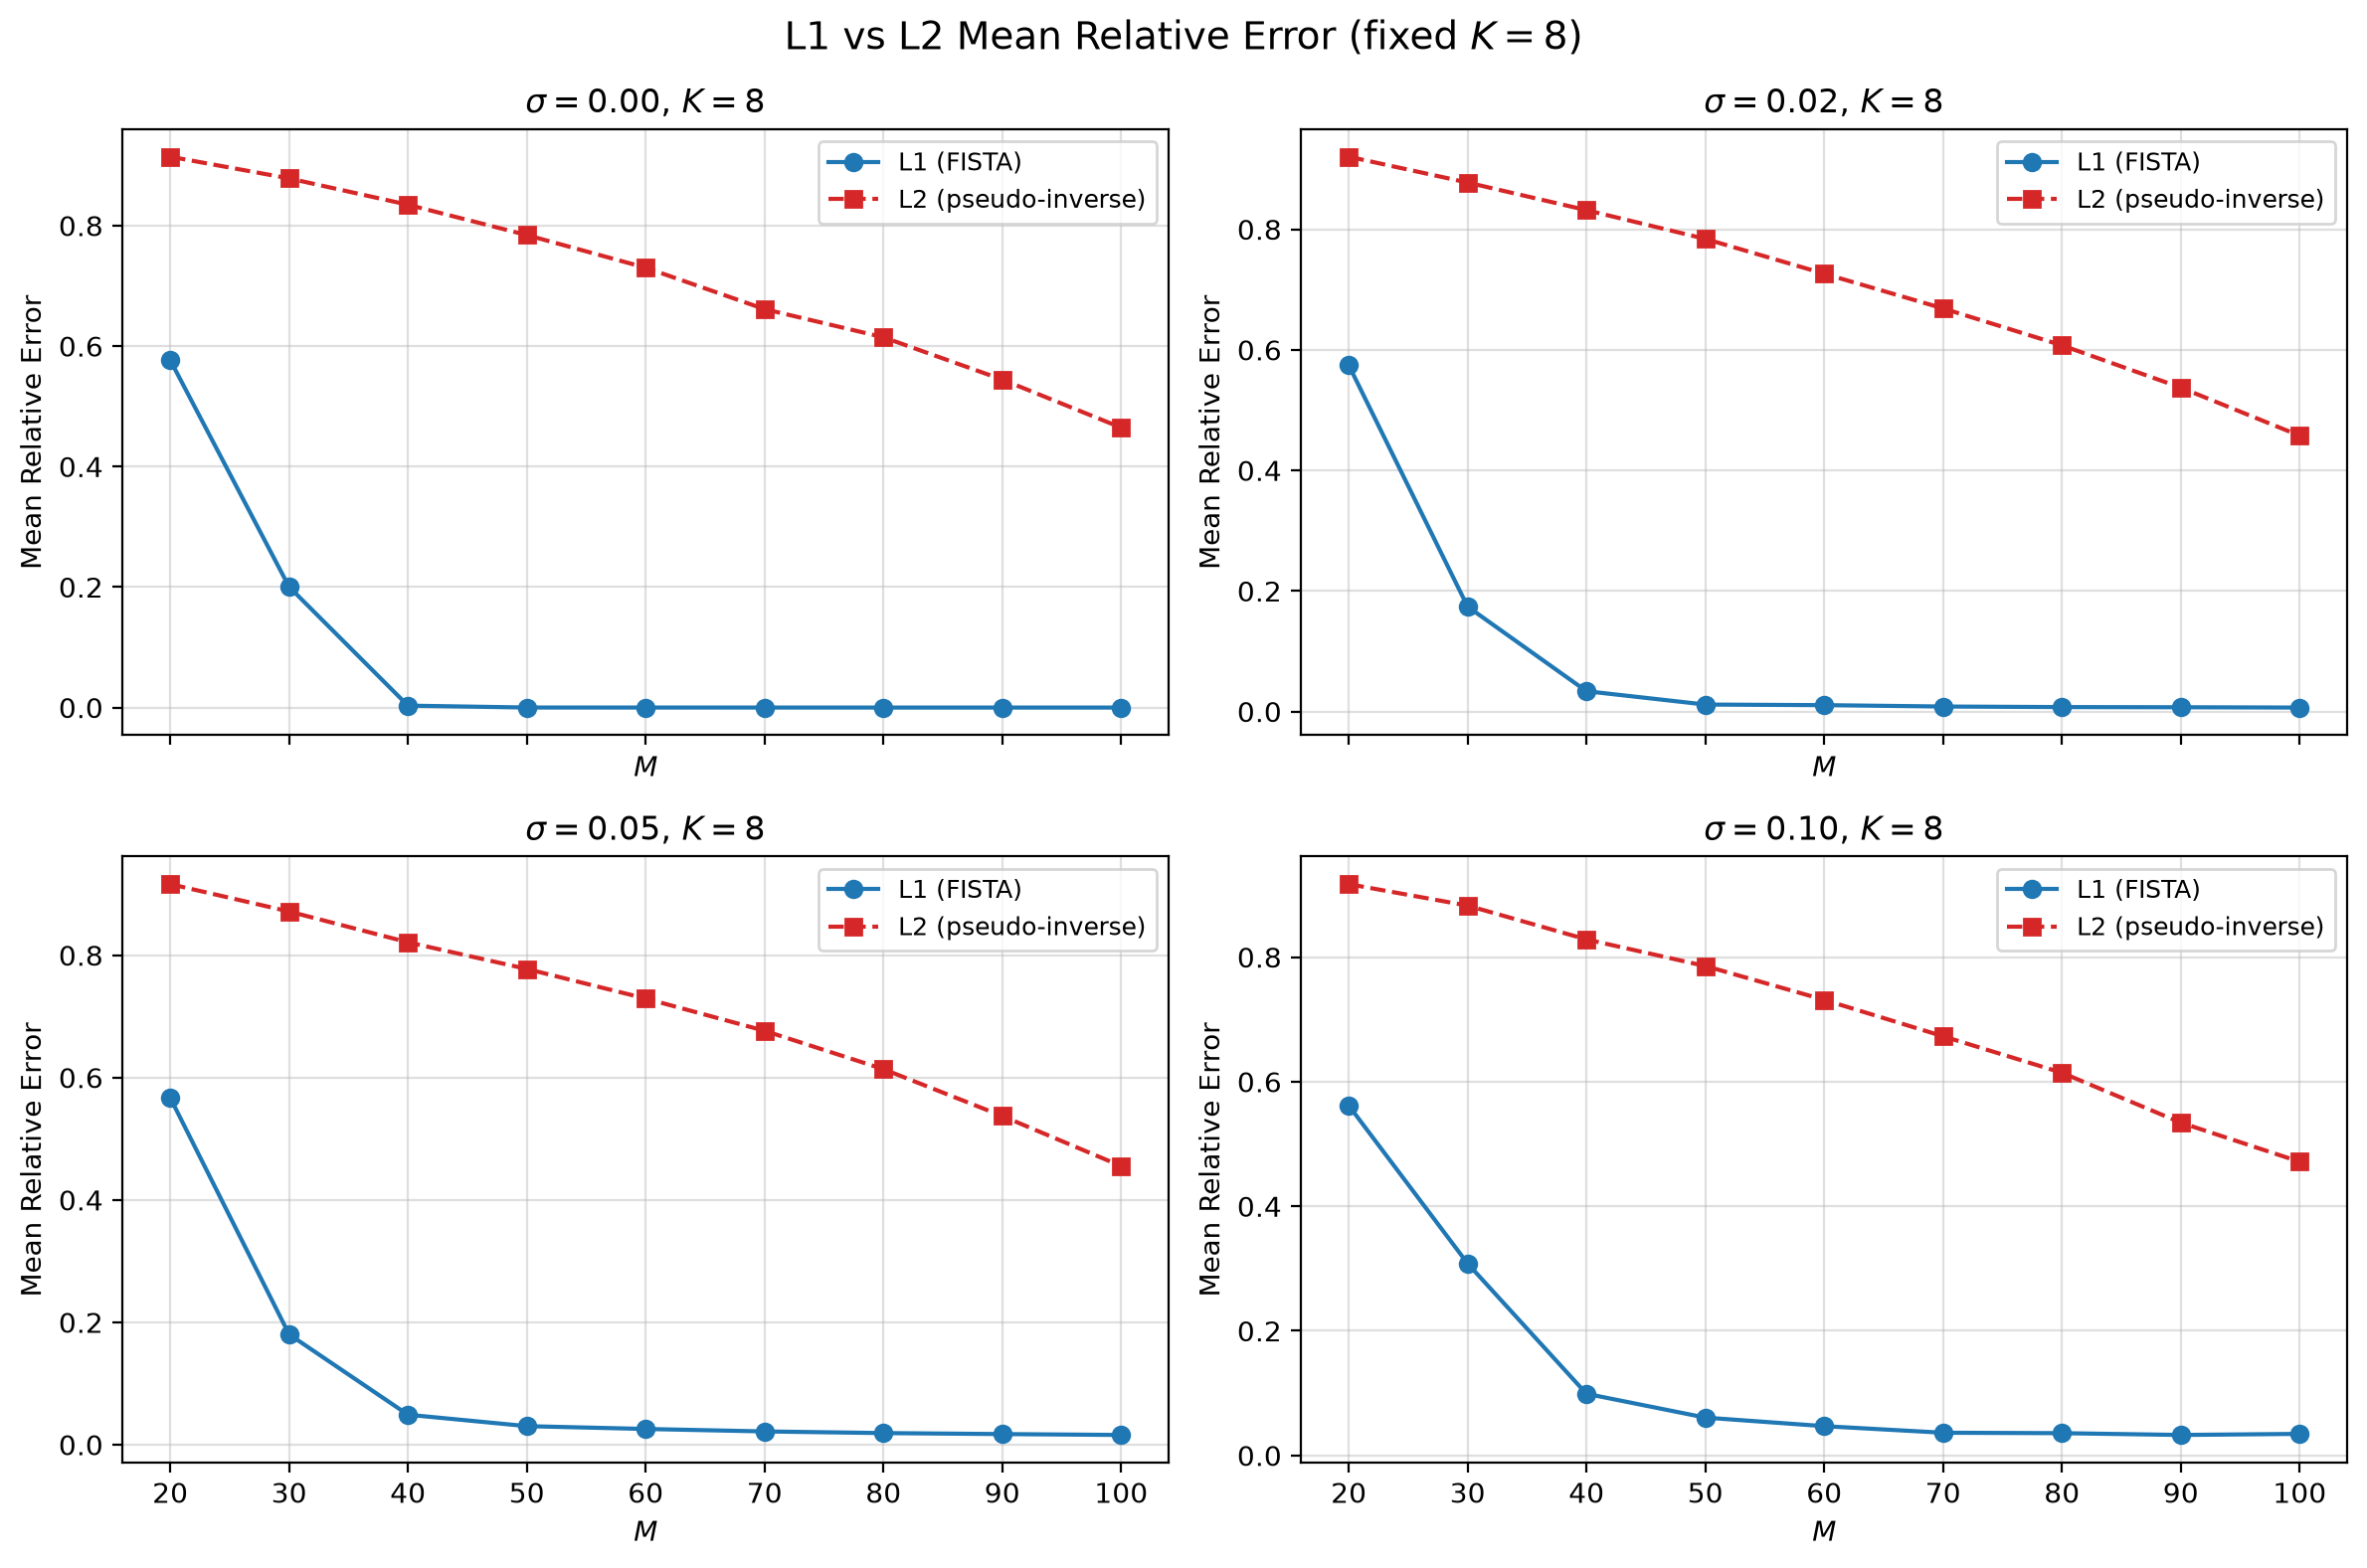
\includegraphics[width=0.9\textwidth]{figures/fig3_re_L1_vs_L2.png}
\caption{固定 $K=8$ 时，L1 与 L2 平均相对重建误差随观测维度 $M$ 的变化对比}
\label{fig:re-compare}
\end{figure}

\begin{figure}[H]
\centering
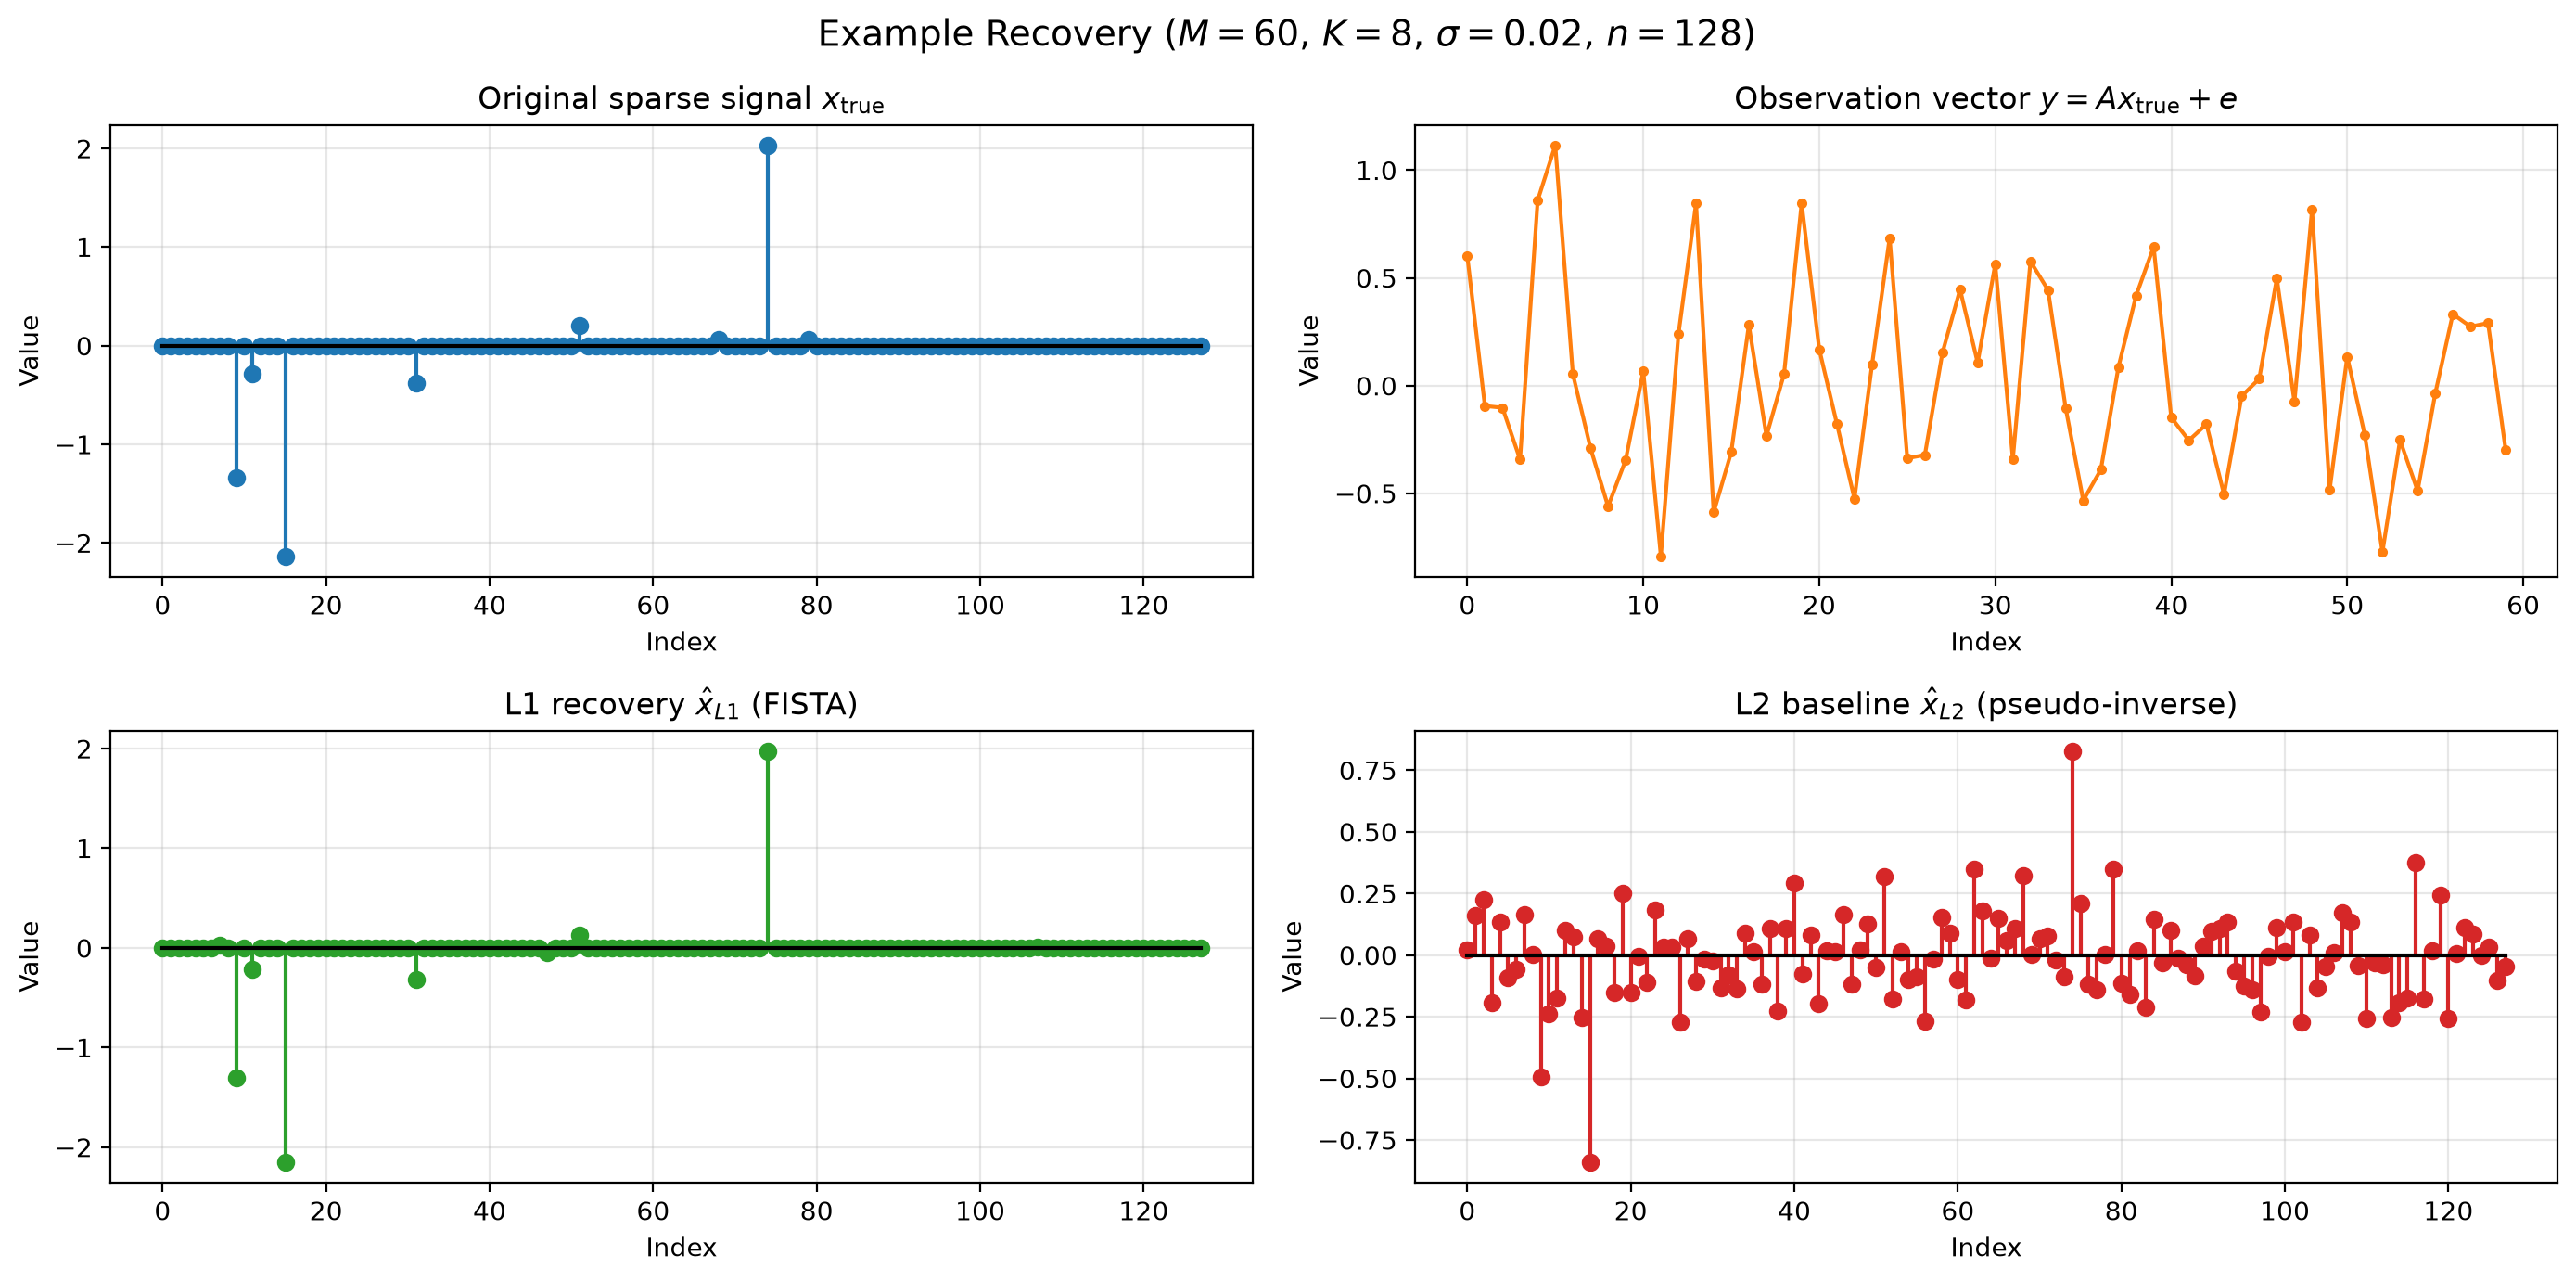
\includegraphics[width=0.96\textwidth]{figures/fig4_sample_recovery.png}
\caption{单次样例恢复对照（$M=60$，$K=8$，$\sigma=0.02$，$n=128$）}
\label{fig:sample}
\end{figure}

\section{结果分析与讨论}
\label{sec:results}

本章基于第 6 章生成的四类图表，从稀疏恢复相变现象、三参数影响规律、与 RIP 理论下界的对比以及误差来源四个方面对仿真结果进行分析。

\subsection{稀疏恢复相变现象}
\label{sec:phase-transition}

图 6-1 给出了无噪声情形（$\sigma=0$）下 L1 支撑集恢复成功率随观测维度 $M$ 与稀疏度 $K$ 变化的热力图。图中存在一条明显的相变带：在低 $M$、高 $K$ 区域成功率接近于 $0$，随着 $M$ 增大、$K$ 减小，成功率迅速过渡到接近 $100\%$。例如，当 $K=3$ 时，$M=20$ 的成功率已达 $92\%$，$M\ge30$ 后稳定为 $100\%$；当 $K=8$ 时，$M=30$ 的成功率仅为 $44\%$，$M=40$ 时跃升至 $98\%$，$M\ge50$ 后保持 $100\%$；当 $K=20$ 时，$M=50$ 的成功率仅为 $12\%$，$M=60$ 时为 $64\%$，$M=70$ 后才达到 $100\%$。

若记临界观测维度 $M^*$ 为成功率首次达到 $100\%$ 的最小 $M$，则 $M^*$ 随 $K$ 的增大而单调增大。图 6-2 的折线图进一步表明，固定 $K$ 时成功率随 $M$ 呈明显的 $S$ 型上升；$K$ 越大，整条曲线越向右移动，说明需要更多的观测才能实现可靠恢复。该现象与压缩感知理论中“存在相变临界值”的预期一致。

\subsection{三参数影响规律}
\label{sec:param-effects}

\paragraph*{稀疏度 $K$ 的影响}
在相同噪声水平下，$K$ 越大，达到可靠恢复所需的观测维度越高。以 $\sigma=0$ 为例，$K=3$ 在 $M=30$ 时即可达到 $100\%$ 成功率，$K=8$ 需要 $M=40$，而 $K=20$ 需要 $M=70$。这说明信号越稀疏，越容易从少量观测中恢复；稀疏度增加会显著提高恢复难度。

\paragraph*{观测维度 $M$ 的影响}
随着 $M$ 增大，支撑集恢复成功率总体上升，平均相对重建误差下降。在可恢复区域内，L1 方法的相对重建误差迅速降至接近 $0$（无噪声时可达 $10^{-4}$ 量级以下）；而在欠采样区域，误差较高且恢复不稳定。

\paragraph*{噪声强度 $\sigma$ 的影响}
噪声会同时降低成功率和重建精度。以 $K=8$、$M=40$ 为例，$\sigma=0,0.02,0.05,0.10$ 时的 L1 成功率分别为 $98\%,80\%,74\%,36\%$。图 6-3 显示，随着 $\sigma$ 增大，L1 误差曲线在中等 $M$ 区域的下降速度变慢，最终误差下限也被抬高；相变临界观测维度整体向右移动。

\subsection{与 RIP 理论下界对比}
\label{sec:rip-comparison}

RIP 理论给出稀疏恢复的充分条件~\scite{candes2005decoding}
\begin{equation}
\label{eq:rip-bound}
M\ge C K\log\left(\frac{n}{K}\right),
\end{equation}
其中 $C$ 为常数。需要强调的是，RIP 条件给出的是恢复的充分条件，且其针对的是测量矩阵满足 RIP 这一事件；而实验中统计的是支撑集恢复成功率 $\Pr(\hat{S}=S_{\mathrm{true}})$，两者并不是同一个随机变量或事件，因此不能直接从实验临界点反推出 RIP 常数 $C$。

不过，可以基于经验恢复阈值对 $C K\log(n/K)$ 进行数量级比较。例如在无噪声热力图中，取成功率首次达到约 $95\%$ 以上的临界观测维度 $M^*$，可观察到 $M^*$ 随 $K$ 增大而增大，且与 $K\log(n/K)$ 大致保持同一数量级：对 $K=5,8,16,20$，$M^*/\left(K\log(n/K)\right)$ 分别约为 $1.85,1.80,1.80,1.89$。这说明实验临界采样规模与 RIP 理论尺度一致，但上述比值不应被解释为对 RIP 常数 $C$ 的估计。

此外，噪声会使所需 $M$ 进一步增大，因此有噪声情形下的临界采样规模会整体右移。

\subsection{误差与性能偏差来源分析}
\label{sec:error-sources}

仿真结果与理论理想情况存在一定偏差，主要来源包括：

\begin{itemize}
\item \textbf{随机矩阵的 RIP 性质}：高斯随机矩阵仅以高概率满足 RIP，并非每次随机试验都能保证恢复条件成立，因此个别试验可能失败；
\item \textbf{观测噪声}：噪声带来不可避免的重建误差，即使支撑集被正确恢复，相对重建误差也存在一个正的下界；
\item \textbf{数值迭代精度}：FISTA 存在有限迭代次数和收敛阈值，$\lambda$ 路径插值也只能近似满足残差约束 $\|Ax-y\|_2=\delta$，这些都会引入微小数值误差；
\item \textbf{L1 凸松弛的充分非必要性}：L1 松弛是 L0 问题的凸近似，存在部分信号无法通过 L1 精确恢复，这是方法本身的固有局限；
\item \textbf{阈值选取}：$\delta$ 取卡方分布的高概率上界，可能略大于真实噪声水平，导致约束偏松、解偏稀疏，也会影响恢复精度。
\end{itemize}

这些因素共同造成了成功率并非严格 $0/1$ 跳变、而是呈现过渡带的现象，也解释了 L1 与 L2 基线之间的显著性能差异。

\section{结论}
\label{sec:conclusion}

本文围绕带噪声稀疏信号恢复问题，从理论、算法和实验三个层面完成了对 L1 凸松弛压缩感知恢复方案的系统研究。

在理论层面，本文建立了带噪声稀疏恢复的约束优化模型，推导了 L1 凸松弛问题的 KKT 条件，验证了 Slater 约束规格与强对偶性，为后续算法设计提供了理论基础。

在算法层面，本文未使用现成凸优化求解器，自主实现了 FISTA 加速近端梯度算法；针对约束形式 L1 恢复，设计了 $\lambda$ 几何递减序列与残差曲线插值策略，稳健匹配残差约束 $\delta$；同时采用解析伪逆作为 L2 最小范数基线，保证对比公平并降低计算开销。

在实验层面，本文在 $n=128$ 的参数网格上进行了大规模仿真，分析了观测维度 $M$、稀疏度 $K$ 与噪声强度 $\sigma$ 对恢复性能的影响。结果表明：
\begin{itemize}
\item L1 恢复存在明显的相变现象，存在临界观测维度 $M^*$，当 $M$ 超过 $M^*$ 时支撑集恢复成功率快速趋近 $100\%$；
\item 稀疏度 $K$ 越大，所需观测维度越高；噪声强度 $\sigma$ 越大，相变临界右移，重建误差上升；
\item 与 L2 最小范数基线相比，L1 方法在支撑集恢复成功率和相对重建误差两个指标上均显著占优，验证了稀疏先验在欠定线性逆问题中的关键作用。
\end{itemize}

综上，本文从理论推导、自研算法到数值实验，完整验证了 L1 凸松弛结合 FISTA 的稀疏恢复方案的有效性与稳健性。

\begin{thebibliography}{9}

\bibitem{donoho2006}
D.~L. Donoho.
Compressed sensing.
\emph{IEEE Transactions on Information Theory}, 52(4):1289--1306, 2006.

\bibitem{candes2006stable}
E.~J. Cand\`es, J.~K. Romberg, and T.~Tao.
Stable signal recovery from incomplete and inaccurate measurements.
\emph{Communications on Pure and Applied Mathematics}, 59(8):1207--1223, 2006.

\bibitem{boyd2004}
S.~Boyd and L.~Vandenberghe.
\emph{Convex Optimization}.
Cambridge University Press, 2004.

\bibitem{beck2009}
A.~Beck and M.~Teboulle.
A fast iterative shrinkage-thresholding algorithm for linear inverse problems.
\emph{SIAM Journal on Imaging Sciences}, 2(1):183--202, 2009.

\bibitem{candes2005decoding}
E.~J. Cand\`es and T.~Tao.
Decoding by linear programming.
\emph{IEEE Transactions on Information Theory}, 51(12):4203--4215, 2005.

\end{thebibliography}

\end{document}
